% 2016 年全国卷Ⅱ理科第 22 题：正方形内的垂足与连线
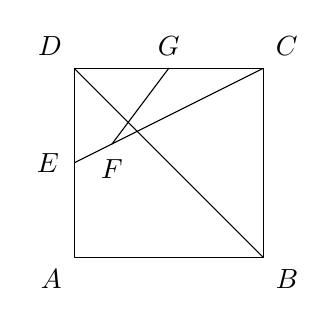
\begin{tikzpicture}[line cap=round,line join=round]
  \coordinate (A) at (0,0);
  \coordinate (B) at (2.4,0);
  \coordinate (C) at (2.4,2.4);
  \coordinate (D) at (0,2.4);
  \coordinate (E) at (0,1.2);
  \coordinate (G) at (1.2,2.4);
  \coordinate (F) at (0.48,1.44);

  \draw (A)--(B)--(C)--(D)--cycle;
  \draw (D)--(B);
  \draw (E)--(C);
  \draw (F)--(G);

  \node[below left=1pt] at (A) {$A$};
  \node[below right=1pt] at (B) {$B$};
  \node[above right=1pt] at (C) {$C$};
  \node[above left=1pt] at (D) {$D$};
  \node[left=2pt] at (E) {$E$};
  \node[above=1pt] at (G) {$G$};
  \node[below=2pt] at (F) {$F$};
\end{tikzpicture}
